
\chapter{研究 : 3次元一様有限温度系のゼロモード}
2015年度夏の学校. 有限温度ゼロモード系における自己無撞着計算がメイン. 有限温度系で重要な計算や考え方が頻出.

また, 夏の学校時点では凝縮粒子数の定義にゼロモード演算子の期待値を加えていなかったため, Depletionは相互作用定数$g$が小さいところで持ち上がる結果を得た. 凝縮粒子数の定義を変えたところ, Depletionは相互作用定数$g$に対してロバストになった. こっちのほうが自然だろうというのが今のところの結論. 
\section{問題設定}
粒子間の相互作用を考慮に入れてゼロモード演算子の期待値を計算をする.この効果のことを量子補正と呼ぶ.\\
相互作用がある場合はゼロ温度でも全ての粒子が凝縮するわけではないことから,今回は主に凝縮粒子数と非凝縮粒子数の割合(depletion)が相互作用によってどのように変わるか,またゼロモードの寄与がある場合とない場合で結果がどのように変わるかを見る.

まずは,量子補正を考慮した方程式の定式化から入る.
\subsection{冷却原子気体系のハミルトニアン}
冷却原子気体のハミルトニアンは以下のように与えられる.
\begin{eqnarray}
  H_{\rm H}=\int d\bm{x}\left[\psi_{\rm H}^\dagger(h_0-\mu)\psi_{\rm H} +\frac{g}{2}\psi_{\rm H}^\dagger\psi_{\rm H}^\dagger\psi_{\rm H}\psi_{\rm H}\right]
\end{eqnarray}
添字のHはHeisenberg描像であることを示している.$\mu$は化学ポテンシャル,$g$は相互作用定数,$h_0$は
\begin{eqnarray}
  h_0 = -\frac{\nabla^2}{2m}
\end{eqnarray}
であるような一様系を取り扱う.場の演算子$\psi_{\rm H}$は同時刻交換関係
\begin{eqnarray}
  &&\left[\psi_{\rm H}(\bm{x},t),\psi_{\rm H}^\dagger(\bm{x}',t) \right] = \delta(\bm{x} - \bm{x}')\\
  &&\left[\psi_{\rm H}(\bm{x},t),\psi_{\rm H}(\bm{x}',t) \right] = 0,\ \ \ \ \ \left[\psi_{\rm H}^\dagger(\bm{x},t),\psi_{\rm H}^\dagger(\bm{x}',t) \right] = 0
\end{eqnarray}
を満たす.このとき,$\psi_{\rm H}$は真空期待値を持つ:
\begin{eqnarray}
  \langle 0|\psi_{\rm H}(\bm{x})|0\rangle = \xi(\bm{x})\label{vaccum_ex1}
\end{eqnarray}
$\xi$は秩序変数と呼ばれ,$|\xi|^2$は凝縮体の密度と解釈できる.秩序変数は今回は時間に依存しないと仮定する.
場の演算子を以下のように分割する:
\begin{eqnarray}
  \psi_{\rm H} = \xi + \varphi_{\rm H}
\end{eqnarray}
$\xi$は凝縮体を記述する古典場,$\varphi_{\rm H}$は非凝縮体を記述する場の演算子と解釈できる.これは同時刻交換関係
\begin{eqnarray}
  \left[\varphi_{\rm H}(\bm{x},t),\varphi^\dagger_{\rm H}(\bm{x}',t)\right]  = \delta(\bm{x}-\bm{x}')\label{equal_time_commutation}
\end{eqnarray}
を満たしている.

ハミルトニアンを$\varphi_{\rm H}$の次数について整理すると
\begin{eqnarray}
  &&H_{{\rm H},1} = \int d\bm{x}\left[\varphi^\dagger_{\rm H}(h_0 - \mu + g|\xi|^2)\xi + \varphi_{\rm H}(h_0 - \mu + g|\xi|^2)\xi^*\right]\\
  &&H_{{\rm H},2} = \int d\bm{x}\left[\varphi^\dagger_{\rm H} {\cal L}\varphi_{\rm H} + \frac{1}{2}\varphi_{\rm H}{\cal M^*}\varphi_{\rm H}+\frac{1}{2}\varphi^\dagger_{\rm H}{\cal M}\varphi^\dagger_{\rm H}\right]\\
  &&H_{{\rm H},3} = g\int d\bm{x}\left[\xi^*\varphi^\dagger_{\rm H}\varphi_{\rm H}\varphi_{\rm H} + \xi\varphi^\dagger_{\rm H}\varphi^\dagger_{\rm H}\varphi_{\rm H} \right] \\
  &&H_{{\rm H},4} = \frac{g}{2}\int d\bm{x}\ \varphi^\dagger_{\rm H}\varphi^\dagger_{\rm H}\varphi_{\rm H}\varphi_{\rm H}
\end{eqnarray}
であり
\begin{eqnarray}
  {\cal L} = h_0 - \mu +2g|\xi|^2,\ \ \ \ \ {\cal M}=g\xi^2
\end{eqnarray}
である.

\subsection{相互作用描像}
系が十分低温であり相互作用$g$が小さいとする.この場合$H_{{\rm H},3},H_{{\rm H},4}$の効果は小さいとして,非摂動ハミルトニアンを$H_{{\rm H},u}=H_{{\rm H},1}+H_{{\rm H},2}$のように選び,Heisenberg描像から相互作用描像に移行する.まず
\begin{eqnarray}
  i\frac{d}{dt}U(t,t_0)=U(t,t_0)H_{{\rm H},p},\ \ \ \ \ U(t_0,t_0)=1,\ \ \ \ \ H_{{\rm H},p} = H_{\rm H} - H_{{\rm H},u}
\end{eqnarray}
を満たすようなユニタリー演算子$U(t,t_0)$を考え,Heisenberg描像の任意の演算子$A_{\rm H}(t)$を用いて相互作用描像の演算子を
\begin{eqnarray}
  A(t) = U(t,t_0)A_{\rm H}(t)U^{-1}(t,t_0)
\end{eqnarray}
と定義する.$t_0$はHeisenberg描像と相互作用描像が一致する時間である.Heisenberg方程式は
\begin{eqnarray}
  i\frac{d}{dt}A(t) = \left[A(t),H_u(t)\right]
\end{eqnarray}
である.ここで$A=H_u$と代入すると時間に依存しないことがわかるので,$H_u = H_{{\rm H},u}$である.

$U(t,t_0)$の時間発展は$H_{{\rm H},p}=H_{{\rm H},3}+H_{{\rm H},4}$に依存し,かつその効果が小さいことから場の演算子の摂動ゼロ次は
\begin{eqnarray}
  \langle0|\varphi_{\rm H}(x)|0\rangle = \langle0| U^{-1}(t,t_0)\varphi(x)U(t,t_0)|0\rangle \simeq \langle0|\varphi(x)|0\rangle
\end{eqnarray}
となっている.また相互作用描像のHeisenberg方程式より
\begin{eqnarray}
  i\frac{\partial}{\partial t}\varphi(x) = \left[\varphi(x),H_u\right]\label{Heisenberg}
\end{eqnarray}
であることがわかる.これ以降$x=(\bm{x},t)$とする.つまり,場の分割条件を
\begin{eqnarray}
  \langle0|\varphi_{\rm H}(x)|0\rangle \simeq \langle0|\varphi(x)|0\rangle = 0
\end{eqnarray}
とした場合,この性質が保存するためには式(\ref{Heisenberg})より
\begin{eqnarray}
  \bra{0}\left[\varphi(x),H_u\right]\ket{0} = 0
\end{eqnarray}
が必要となる.ここから定常Gross-Pitaevskii方程式(GP方程式)
\begin{eqnarray}
  \left[h_0 - \mu +g|\xi|^2\right]\xi = 0\label{GP}
\end{eqnarray}
が導かれる.
\subsection{量子補正}
量子補正を取り入れる場合は場の分割条件を$\bra{0}[\varphi,H_u]\ket{0}=0$ではなく
\begin{eqnarray}
  \bra{0}[\varphi,H]\ket{0} = 0 \label{split}
\end{eqnarray}
とする.これはもともとの場の分割条件$\bra{0}\varphi_H\ket{0} = 0$の摂動1次までを取り入れたことになっている\footnote{実は正確な表現ではない. }.これを具体的に計算する:
\begin{eqnarray}
  \nonumber  \bra{0}[\varphi,H_1]\ket{0} &=& \bra{0}\int d\bm{x}\left[\varphi,\left\{\varphi^\dagger{\cal L}\xi+\varphi{\cal L}\xi^*\right\}\right]\ket{0}\\
  &=& (h_0 - \mu + g|\xi|^2)\xi\\
  \nonumber  \bra{0}[\varphi,H_2]\ket{0} &=& \bra{0}\int d\bm{x}\left[\varphi,\left\{\varphi^\dagger{\cal L}\varphi+\frac{1}{2}\varphi{\cal M}^*\varphi + \frac{1}{2}\varphi^\dagger{\cal M}\varphi^\dagger\right\}\right]\ket{0}\\
  &=& \bra{0}{\cal L}\varphi + {\cal M}\varphi^\dagger \ket{0} = 0\\
  \nonumber  \bra{0}[\varphi,H_3]\ket{0} &=& \bra{0}g\int d\bm{x}\left[\varphi,\left\{\xi^*\varphi^\dagger\varphi\varphi + \xi\varphi^\dagger\varphi^\dagger\varphi \right\}\right]\ket{0}\\
  &=& g\bra{0}\varphi\varphi\ket{0}\xi^* + 2g\bra{0}\varphi^\dagger\varphi\ket{0}\xi\\
  \nonumber  \bra{0}[\varphi,H_4]\ket{0} &=& \bra{0}\frac{g}{2}\int d\bm{x}\left[\varphi,\varphi^\dagger\varphi^\dagger\varphi\varphi\right]\ket{0}\\
  &=& g\bra{0}\varphi^\dagger\varphi\varphi\ket{0}
\end{eqnarray}
ここで$\varphi$の3次の期待値の寄与は小さいものとすると,式(\ref{split})より
\begin{eqnarray}
  \left[h_0 - \mu + g|\xi|^2 + 2g\bra{0}\varphi^\dagger\varphi\ket{0}\right]\xi + g\bra{0}\varphi\varphi\ket{0}\xi^* = 0
\end{eqnarray}
これが量子補正を考慮したGP方程式である.ここでゼロモード部と励起部に分けて記述すると
\begin{eqnarray}
 \nonumber \bra{0}\varphi^\dagger\varphi\ket{0} &=& _{\rm ex}\bra{0}\varphi^\dagger_{\rm ex}\varphi_{\rm ex}\ket{0}_{\rm ex} + |\xi|^2\bra{\Psi}Q^2\ket{\Psi} + |\eta|^2\bra{\Psi}P^2\ket{\Psi} \\
  &&\ \ \ \ \ \ \ \ -{\rm Re}\xi^*\eta -{\rm Im}\xi^*\eta(QP + PQ)\\
\nonumber  \bra{0}\varphi\varphi\ket{0} &=& _{\rm ex}\bra{0}\varphi_{\rm ex}\varphi_{\rm ex}\ket{0}_{\rm ex} - \xi^2\bra{\Psi}Q^2\ket{\Psi} + \eta^2\bra{\Psi}P^2\ket{\Psi} \\
  &&\ \ \ \ \ \ \ \ -i\xi\eta\bra{\Psi}QP + PQ\ket{\Psi}
\end{eqnarray}
となる.ここで$\varphi = -iQ\xi + P\eta + \varphi_{\rm ex}$とし,かつ$\ket{0} = \ket{0}_{\rm ex}\otimes\ket{\Psi}$としている.$Q,P$は正準交換関係$[Q,P] = i$を満たすゼロモード演算子,非摂動ハミルトニアン$H_u$の励起部$H_u^{\rm ex}$,ゼロモード部$H_u^{QP}$の固有状態をそれぞれ$\ket{0}_{\rm ex},\ket{\Psi}$である.

GP方程式が補正を受けたので,Bogoliubov-de Gennes方程式(BdG方程式)にも補正を加える.具体的には
\begin{eqnarray}
  {\cal L} &=&  h_0 - \mu + 2g(|\xi|^2 + \bra{0}\varphi^\dagger\varphi\ket{0})\label{L}\\
  {\cal M} &=& g(\xi^2 - \bra{0}\varphi\varphi\ket{0})\label{M}
\end{eqnarray}
となっていれば$\bm{y}_0 = \begin{pmatrix}\xi & -\xi^*  \end{pmatrix}$がゼロモードであることを守れる.ここで非摂動ハミルトニアンを
\begin{eqnarray}
  H_u = H_1 + H_2 + [H_3 + H_4]_{QP} -\delta\mu P -\delta\nu Q + \delta H
\end{eqnarray}
と取り,カウンター項$\delta H$を
\begin{eqnarray}
  \delta H = g\int d\bm{x}\left[2\varphi^\dagger\varphi\bra{0}\varphi^\dagger\varphi\ket{0}-\frac{1}{2}\varphi\varphi\bra{0}\varphi^\dagger\varphi^\dagger\ket{0}-\frac{1}{2}\varphi^\dagger\varphi^\dagger\bra{0}\varphi\varphi\ket{0}\right]
\end{eqnarray}
と選ぶことで,$H_u^{QP}$は量子補正を考慮しない場合と同じ形を取ることができる.式(\ref{L})(\ref{M})より共役モード方程式$
\begin{pmatrix}
  {\cal L} & {\cal M}\\
  -{\cal M}&-{\cal L}
\end{pmatrix}
\bm{y}_{-1}=I\bm{y}_0
$は
\begin{eqnarray}
  \left[h_0 - \mu + 2g(|\xi|^2 + \bra{0}\varphi^\dagger\varphi\ket{0})\right]\eta + g(\xi^2 - \bra{0}\varphi\varphi\ket{0})\eta^*=I\xi
\end{eqnarray}
となる.以上の定式化を用いて各物理量の計算を行っていく.
\section{自己無撞着ループ}
前節で導いた関係式に現れる物理量は自己無撞着に決定されるが,その関係式同士のつながりは複雑である.
以下では3次元一様有限温度系に現れる自己無撞着ループについてまとめる.2章のはなしを有限温度に拡張するために期待値のとり方を変えていることに注意.
\\

\begin{itembox}[c]{0. 初期設定}
  \begin{center}
    $V_t = \ev{\varphi^{\dagger}\varphi} = 0$, $V_a = \ev{\varphi\varphi} = 0$からスタート
  \end{center}
\end{itembox}

\begin{center}
  $\Downarrow$
\end{center}

\begin{itembox}[c]{1. GP方程式}
  \begin{center}
    GP方程式より$\xi, \mu $を求める
  \end{center}
\end{itembox}

\begin{center}
  $\Downarrow$
\end{center}

\begin{itembox}[c]{2. 共役モード方程式}
  \begin{center}
    共役モード方程式より$\eta, I$を求める
  \end{center}
\end{itembox}

\begin{center}
  $\Downarrow$
\end{center}

\begin{itembox}[c]{3. BdG方程式}
  \begin{center}
    BdG方程式(Bogoliubov変換)より$u_l, v_l$を求める
  \end{center}
\end{itembox}

\begin{center}
  $\Downarrow$
\end{center}

\begin{itembox}[c]{4. ゼロモード方程式}
  \begin{center}
    ゼロモード方程式より固有関数$\ev{q|\Psi}$を求め,$\ev{P}$を求める\\
    $\Updownarrow$\\
    $\ev{P} = 0$となるように自己無撞着に$\delta\mu$を決定
  \end{center}
\end{itembox}

\begin{center}
  $\Downarrow$
\end{center}

\begin{itembox}[c]{5. ゼロモード演算子}
  \begin{center}
    $\ev{Q^2}, \ev{P^2}$を求める
  \end{center}
\end{itembox}

\begin{center}
  $\Downarrow$
\end{center}

\begin{itembox}[c]{6. 熱平均・異常平均}
  \begin{center}
    $V_t, V_a$を求める.
  \end{center}
\end{itembox}

\begin{center}
  $\Downarrow$
\end{center}

\begin{itembox}[c]{ループ/終了条件}
  \begin{center}
    「1. GP方程式」 に戻って計算を繰り返す.$V_t, V_a$の値が変化しなくなったら終了.
  \end{center}
\end{itembox}

\subsection{GP方程式}
入力:$V_t,V_a$

$\xi,\eta$は実数とする.量子補正を含むGP方程式は
\begin{eqnarray}
  [-\mu + g\xi^2 + g(2V_t + V_a)]\xi = 0
\end{eqnarray}  
である.今回は一様系を扱うため微分項$h_0$がなくなり,簡単な代数方程式になる.これを$\mu$について解く:
\begin{eqnarray}
  \mu = g(\xi^2 + 2V_t + V_a)
\end{eqnarray}
ここで粒子数$N$が保存するためには
\begin{eqnarray}
  \nonumber  N &=& \int d\bm{x}\ev{\psi^\dagger\psi}\\
  \nonumber  &=& \int d\bm{x}\ev{(\xi + \varphi^\dagger)(\xi + \varphi)}\\
  &=& V(\xi^2 + V_t)
\end{eqnarray}
を満たさなければならない.ここでは分割条件から$\ev{\varphi},\ev{\varphi^\dagger}$はゼロになっている.したがって,
\begin{itembox}[c]{GP方程式}
\begin{eqnarray}
  \xi &=& \sqrt{\frac{N}{V} - V_t}\\
  \mu &=& g(\frac{N}{V} + V_t + V_a)
\end{eqnarray}
\end{itembox}
となることがわかる.

\subsection{共役モード方程式}
入力:$V_a, V_t, \xi, \mu$

量子補正を含む共役モード方程式は
\begin{eqnarray}
  [-\mu + g(3\xi^2 + 2V_t - V_a)]\eta = I\xi 
\end{eqnarray}
である.GP方程式と同様の理由で代数方程式となっている.これを$I$について解く:
\begin{eqnarray}
  I = \frac{\eta}{\xi}[-\mu + g(3\xi^2 + 2V_t - V_a)]
\end{eqnarray}
ここでゼロモードと共役モードの規格化条件から
\begin{eqnarray}
  \nonumber  (\bm{y}_0, \bm{y}_{-1}) &=& \int d\bm{x}
  \begin{pmatrix}
    \xi & -\xi
  \end{pmatrix}
  \begin{pmatrix}
    1 & 0\\
    0 & -1
  \end{pmatrix}
  \begin{pmatrix}
    \eta\\
    \eta
  \end{pmatrix}\\
  &=& 2V\xi\eta = 1
\end{eqnarray}
を満たさなければならない.したがって
\begin{itembox}[c]{共役モード方程式}
\begin{eqnarray}
  \eta &=& \frac{1}{2V\xi}\\
  I &=& \frac{-\mu + g(3\xi + 2V_t - V_a)}{2V\xi^2}
\end{eqnarray}
\end{itembox}
となることがわかる.

\subsection{BdG方程式}
入力:$V_a, V_t, \xi, \mu$

一様系ではBogoliubov変換から$u_l,v_l$を求めることができる.

\begin{eqnarray}
  \varphi = \frac{1}{(2\pi)^{3/2}}\int d\bm{k}\ b_{\bm{k}}e^{i\bm{k}\bm{x}}
\end{eqnarray}
と展開すると,ハミルトニアンの2次$H_2$は
\begin{eqnarray}
  H_2 = \frac{1}{2}\int d\bm{k}\ [2{\cal L}_kb^\dagger_{\bm{k}}b_{\bm{k}} + {\cal M}(b^\dagger_{\bm{k}}b^\dagger_{-\bm{k}} + b_{\bm{k}}b_{-\bm{k}})]
\end{eqnarray}
とかける.ただし
\begin{eqnarray}
  {\cal M} &=& g(\xi^2 - V_a)\\
  \nonumber  {\cal L}_k &=& \frac{\hbar^2}{2m}k^2 - \mu + 2g(\xi^2 + V_t)\\
  &=& \frac{\hbar^2}{2m}k^2 + {\cal M}
\end{eqnarray}
である.ここで
\begin{eqnarray}
  H_2 = \int d\bm{k}\ \omega_ka^\dagger_{\bm k}a_{\bm k}
\end{eqnarray}
となるような
\begin{eqnarray}
  a_{\bm k} = u_kb_{\bm k} - v_kb_{-\bm{k}}\label{operator}
\end{eqnarray}
を満たす$u_k$, $v_k$を探す.$a_k$は生成消滅演算子の代数を満たさなければならないので
\begin{eqnarray}
  |u_k|^2-|v_k|^2=1
\end{eqnarray}
が必要であり,式(\ref{operator})を$b$について解いて$H_2$に代入することにより,対角化の条件は
\begin{eqnarray}
  2{\cal L}_ku_kv_k -{\cal M}(u^2_k + v^2_k) = 0
\end{eqnarray}
であることがわかる.これらを連立させることにより
\begin{itembox}[c]{Bogoliubov変換}
\begin{eqnarray}
  \begin{pmatrix}
      u_k\\
      v_k
    \end{pmatrix}
  &=& \frac{1}{\sqrt{2\omega_k}}
  \begin{pmatrix}
    \sqrt{{\cal L}_k + \omega_k}\\
    -\sqrt{{\cal L}_k - \omega_k}
  \end{pmatrix}\\
  \omega_k &=& \sqrt{{\cal L}^2_k - {\cal M}^2}
\end{eqnarray}
\end{itembox}
を得る.
\subsection{ゼロモード方程式}
入力:\ $\xi, \eta, I$

今回考えるゼロモード方程式は以下:
\begin{eqnarray}
  H_u^{QP}\ket{\Psi_m} = E_m\ket{\Psi_m}
\end{eqnarray}
ただし
\begin{eqnarray}
  \nonumber  H_u^{QP} = -(\delta\mu + 4C)P &+& \frac{I-4D}{2}P^2 + 2BQPQ + 2DP^3\\
  &+& \frac{1}{2}AQ^4 -2BQ^2 + CQP^2Q + \frac{1}{2}EP^4
\end{eqnarray}
である.これを$q$空間で差分化して数値的に解く.$q$空間での波束の幅はおよそ$N_0^{-1/3}$のオーダーであることを基に系のサイズを決める.
\\
\begin{eqnarray}
  \Psi_q = \sqrt{\Delta q}\ev{q|\Psi}
\end{eqnarray}
として差分化すると,ハミルトニアン$H_u^{QP}$は以下のようになる
\begin{eqnarray}
  H_u^{QP} =
  \begin{pmatrix}
    \alpha_0 & \beta_0& \gamma_0& & & \\
    \beta_0^* & \alpha_1 & \beta_1 & \gamma_1 & & \\
    \gamma_0^* &\beta_1^* &\alpha_2 &\beta_2 &\gamma_2 &\\
    &\gamma_1^* & \beta_2^* & \alpha_3 & \ddots & \ddots\\
    & & \gamma_2^* & \ddots &\ddots &\ddots \\
    &&&\ddots &\ddots &\ddots 
  \end{pmatrix}
\end{eqnarray}
\begin{eqnarray}
  \alpha_q &=& \frac{3E}{\Delta q^4} + \frac{I-4D}{\Delta q^2} + (2C -2\Delta q^2B)(q-\frac{N_q}{2})^2 + \frac{\Delta q^4}{2}Aq^4 \\
  \beta_q &=& -\frac{2E}{\Delta q^4} - \frac{2iD}{\Delta q^3} - \frac{I-4D}{2\Delta q^2} + \frac{i(\delta\mu + 4C)}{2\Delta q} - (C + i\Delta qB)(q - \frac{N_q}{2})(q - \frac{N_q}{2}+1)\\
  \gamma_q &=& \frac{E}{2\Delta q^4} + \frac{iD}{\Delta q^3}
\end{eqnarray}
有限温度系での期待値の取り方に注意すると
\begin{eqnarray}
  \nonumber  \ev{P} &=& \frac{{\rm Tr}\rho P}{{\rm Tr}\rho}\\
  \nonumber &=& \frac{\sum_m\bra{\Psi_m} P \ket{\Psi_m}e^{-\beta E_m}}{\sum_me^{-\beta E_m}}\\
  &=& \frac{\sum_m\sum_q{\rm Im} \Psi_q^{*,m}\Psi_{q+1}^me^{-\beta E_m}}{\Delta q\sum_me^{-\beta E_m}}
\end{eqnarray}
ただし密度演算子$\rho$は
\begin{eqnarray}
  \rho = e^{-\beta H_u^{QP}}
\end{eqnarray}
である.場の分割条件から$\ev{P} = 0$を満たさなければならないので,それに合わせて自己無撞着的に$\delta\mu$を決定することになる.数値計算上では二分法を用いる.

\subsection{$\ev{Q^2},\ev{P^2}$の計算}

前節で決定された$\delta \mu$を基に求めたゼロモード固有関数$\Psi^m_q$を用いて$\ev{P}$と同様の計算で$\ev{Q^2},\ev{P^2}$を求める.
\begin{itembox}[c]{ゼロモード演算子の有限温度期待値}
\begin{eqnarray}
  \ev{Q^2}&=& \frac{\Delta q^2\sum_m\sum_q(q - \frac{N_q}{2})|\Psi_q^m|^2e^{-\beta E_m}}{\sum_me^{-\beta E_m}}\\
  \ev{P^2}&=& \frac{2\sum_m\sum_q(|\Psi_q^m|^2-{\rm Re}\Psi_q^{*,m}\Psi_{q+1}^m)e^{-\beta E_m}}{\Delta q^2\sum_me^{-\beta E_m}}
\end{eqnarray}
\end{itembox}

\subsection{熱平均$V_t$・異常平均$V_a$}
入力:$\xi, \eta, u_l, v_l, \ev{Q^2}, \ev{P^2}$

熱平均・異常平均は以下の通り:
\begin{eqnarray}
  V_t = \ev{\varphi^\dagger\varphi} &=& _{{\rm ex}}\ev{\varphi^\dagger_{{\rm ex}}\varphi_{{\rm ex}}}_{{\rm ex}} + \xi^2\ev{Q^2} + \eta^2\ev{P^2} -\xi\eta \\
  %  &=& \sum_l\left[\frac{1}{e^{\beta\omega_l}-1}(|u_l|^2 + |v_l|^2)\right] + \xi^2\ev{Q^2} + \eta^2\ev{P^2} -\xi\eta 
  V_a = \ev{\varphi\varphi} &=& _{{\rm ex}}\ev{\varphi_{{\rm ex}}\varphi_{{\rm ex}}}_{{\rm ex}} - \xi^2\ev{Q^2} + \eta^2\ev{P^2} + i\xi\eta\ev{QP+PQ} 
  %  &=& \sum_l\left[\left(\frac{2}{e^{\beta\omega_l}-1}+1\right)u_lv^*_l\right] - \xi^2\ev{Q^2} + \eta^2\ev{P^2} + i\xi\eta\ev{QP+PQ} 
\end{eqnarray}
$\varphi_{\rm ex}$を以下のように展開する:
\begin{eqnarray}
  \varphi_{\rm ex} = \frac{1}{\sqrt{(2\pi)^3}}\int^{\infty}_{-\infty} d\bm{k}[a_{\bm{k}}u_k + a^\dagger_{-\bm{k}} v_k^*]e^{i\bm{k}\bm{x}}
\end{eqnarray}
ここで$a_{\bm{k}}$が消去する真空を$\ket{0}_k$,粒子数状態を
\begin{eqnarray}
  \ket{n} = \ket{n_1}_1\otimes\ket{n_2}_2\otimes\ket{n_3}_3\otimes... = \underset{k}{\otimes}\ket{n_k}_k
\end{eqnarray}
とする.

以上から$_{\rm ex}\ev{\varphi^\dagger_{{\rm ex}}\varphi_{{\rm ex}}}_{\rm ex},\  _{\rm ex}\ev{\varphi_{{\rm ex}}\varphi_{{\rm ex}}}_{\rm ex}$の計算をしていくために励起モードの期待値計算についてまとめる.
\begin{eqnarray}
  _{\rm ex}\ev{A}_{\rm ex} = \frac{{\rm Tr}\rho A}{{\rm Tr}\rho},\ \ \ \ \ \rho = e^{-\beta H^{\rm ex}_u}
\end{eqnarray}
であり
\begin{eqnarray}
  \nonumber  {\rm Tr}\rho &=& \sum_{n_1}\sum_{n_2}...\bra{n}e^{-\beta\sum_k\omega_{\bm{k}}a^\dagger_{\bm{k}}a_{\bm{k}}}\ket{n} = \sum_{n_1}\sum_{n_2}...\bra{n}e^{-\beta\sum_k\omega_{\bm{k}}n_{\bm{k}}}\ket{n} = \sum_{n_1}\sum_{n_2}...\prod_ke^{-\beta\omega_{\bm{k}}n_{\bm{k}}}\\
  &=& \prod_k\sum_{n_1}\sum_{n_2}...e^{-\beta\omega_{\bm{k}}n_{\bm{k}}} = \prod_k\sum_{n_{\bm{k}}}e^{-\beta\omega_{\bm{k}}n_{\bm{k}}} = \prod_k\frac{1}{1-e^{-\beta\omega_{\bm{k}}}}
\end{eqnarray}
\begin{eqnarray}
  \nonumber  {\rm Tr}\rho a^\dagger_{\bm k}a_{\bm{k}} &=& \sum_{n_1}\sum_{n_2}...\bra{n}e^{-\beta\sum_k\omega_{\bm{k}}a^\dagger_{\bm k}a_{\bm{k}}}a^\dagger_{\bm k}a_{\bm{k}}\ket{n} = \sum_{n_1}\sum_{n_2}...\left(\prod_{l\neq k}e^{-\beta\omega_ln_l}\right)n_le^{-\beta\omega_ln_l}\\
  \nonumber  &=& \prod_{l\neq k}\left(\sum_{n_1}\sum_{n_2}...\sum_{n_{l-1}}\sum_{n_{l+1}}...e^{-\beta\omega_ln_l}\right)\sum_kn_{\bm{k}}e^{-\beta\omega_{\bm{k}}n_{\bm{k}}} = \left(\prod_{k\neq l}\sum_{n_{\bm{k}}}e^{-\beta\omega_ln_l}\right)\sum_kn_{\bm{k}}e^{-\beta\omega_{\bm{k}}n_{\bm{k}}}\\
  &=&\left(\prod_{l\neq k}\frac{1}{1-e^{-\beta\omega_l}}\right)\frac{e^{-\beta\omega_{\bm{k}}}}{(1-e^{-\beta\omega_{\bm{k}}})^2}
\end{eqnarray}
から,
\begin{eqnarray}
  \nonumber  _{\rm ex}\ev{a^\dagger_{\bm{k}}a_{\bm{k}}}_{\rm ex} &=&  \frac{{\rm Tr}\rho a^\dagger_{\bm k}a_{\bm{k}}}{{\rm Tr}\rho}\\
  \nonumber &=& \frac{\left(\prod_{l\neq k}\frac{1}{1-e^{-\beta\omega_l}}\right)\frac{e^{-\beta\omega_{\bm{k}}}}{(1-e^{-\beta\omega_{\bm{k}}})^2}}{\prod_k\frac{1}{1-e^{-\beta\omega_{\bm{k}}}}}\\
  &=&\frac{1}{e^{\beta\omega_{\bm{k}}}-1}\\
  _{\rm ex}\ev{a^\dagger_{\bm{k}}a^\dagger_{-\bm{k}}}_{\rm ex} &=& _{\rm ex}\ev{a_{\bm{k}}a_{-\bm{k}}}_{\rm ex} = 0
\end{eqnarray}
となる.これはBose-Einstein分布関数である. ただし, これは$\bm{k}$が離散の場合である. $\bm{k}$が連続の場合は以下のように拡張する\footnote{付録参照}:
\begin{eqnarray}
  _{\rm ex}\ev{a_{\bm k}^\dagger a_{\bm{k}'}}_{\rm ex} = \frac{1}{e^{\beta\omega_{\bm{k}}}-1}\delta(\bm{k} - \bm{k}')
\end{eqnarray}
これより
\begin{eqnarray}
  \nonumber  _{\rm ex}\ev{\varphi^\dagger_{\rm ex}\varphi_{\rm ex}}_{\rm ex} &=& \frac{1}{(2\pi)^3}\int^{\infty}_{-\infty}  d \bm{k}' d \bm{k}\ {_{\rm ex}\ev{(a_{\bm{k}'}u_{k'}+a^\dagger_{-\bm{k}'}v^*_{k'})^\dagger(a_{\bm{k}}u_k+a^\dagger_{-\bm{k}}v^*_k)}_{\rm ex}}e^{i(\bm{k}-\bm{k}')\bm{x}}\\
  \nonumber  &=& \frac{1}{(2\pi)^3}\int^{\infty}_{-\infty} d \bm{k}' d \bm{k}\left[{_{\rm ex}\ev{a^\dagger_{\bm{k}}a_{\bm{k}}}_{\rm ex}}u^*_ku_k + {_{\rm ex}\ev{a_{-\bm{k}}a^\dagger_{-\bm{k}}}_{\rm ex}}v_kv^*_k\right]\delta(\bm{k}-\bm{k}')e^{i(\bm{k}-\bm{k'})\bm{x}}\\
  &=& \frac{1}{(2\pi)^3}\int^{\infty}_{-\infty} d\bm{k}\left[\frac{1}{e^{\beta\omega_{\bm{k}}}-1}(|u_k|^2+|v_k|^2)+|v_k|^2\right]
\end{eqnarray}
となり,同様の計算により
\begin{eqnarray}
  _{{\rm ex}}\ev{\varphi_{{\rm ex}}\varphi_{{\rm ex}}}_{{\rm ex}} &=& \frac{1}{(2\pi)^3}\int^\infty_{-\infty} d\bm{k}\left[\left(\frac{2}{e^{\beta\omega_k}-1}+1\right){\rm Re}u_kv^*_k\right]
\end{eqnarray}
であることもわかる.ここに$u_k,v_k$の値を代入して$(k_x, k_y, k_z)$から$(k, \theta, \phi)$の変数変換を施すと
\begin{itembox}[c]{熱平均・異常平均}
\begin{eqnarray}
  _{\rm ex}\ev{\varphi^\dagger_{\rm ex}\varphi_{\rm ex}}_{\rm ex} &=& \frac{1}{(2\pi)^2} \int^{\infty}_0 dk\ \frac{k^2}{\omega_k}\left[\frac{2\Lk}{e^{\beta\omega_k} - 1} + \Lk - \omega_k\right]\\
  _{\rm ex}\ev{\varphi_{\rm ex}\varphi_{\rm ex}}_{\rm ex} &=& -\frac{1}{(2\pi)^2} \int^{\infty}_0 dk\ \frac{k^2\M}{\omega_k}\left[\frac{2}{e^{\beta\omega_k}-1}+1\right]
\end{eqnarray}
\end{itembox}
であることがわかる.これらをSimpson積分することで$V_t,\ V_a$を計算する.
\subsubsection{積分範囲の設定}
数値計算上では無限大の積分は不可能なので,適当な値で積分を打ち切る必要がある.$_{\rm ex}\ev{\varphi^\dagger_{\rm ex}\varphi_{\rm ex}}_{\rm ex}$の被積分関数は遠方で収束するので問題ない一方,$_{\rm ex}\ev{\varphi_{\rm ex}\varphi_{\rm ex}}_{\rm ex}$では被積分関数第2項の影響より紫外発散が生じる.これを除去するためにBose-Einstein分布が収束する領域では粒子密度が希薄であることを考慮して第一項が収束する程度までを積分範囲とする.

なお,量子補正を考慮したゼロ温度系の計算をする場合は励起モードが存在しないため,どのような正当性をもって積分範囲を限定するかが自明ではない.現状では逆温度$\beta$が$10^6$程度の極低温の場合の計算とフィットするように積分範囲を決めている.

\subsection{比熱・圧力}
ゼロモードを含めた全エネルギーを{\cal E}とすると,比熱$C_V$, 圧力$P$はぞれぞれ以下の通り:
\begin{eqnarray}
\nonumber  C_V = \frac{\partial {\cal E}_{\rm total}}{\partial T} &=& \frac{\partial}{\partial T}\left[\int d\bm{k} {_{\rm ex}\ev{a^\dagger_{\bm k} a_{\bm k}}_{\rm ex}} + \ev{H_u^{QP}} \right]\\
&=& \frac{\partial}{\partial T}\left[4\pi\int dk \frac{k^2\omega_k}{e^{\beta\omega_k}-1} + \frac{\sum_m E_me^{-\beta E_m}}{\sum_m e^{-\beta E_m}}\right]\\
P = -\frac{\partial {\cal E}_{\rm total}}{\partial V} &=& -\frac{\partial}{\partial V}\left[4\pi\int dk \frac{k^2\omega_k}{e^{\beta\omega_k}-1} + \frac{\sum_m E_me^{-\beta E_m}}{\sum_m e^{-\beta E_m}}\right]
\end{eqnarray}
\section{変分法による見積もり}
ゼロモード演算子の期待値$\ev{Q^4},\ \ev{Q^2},\ \ev{P^2}$の値を変分計算で見積もる.
\subsection{ゼロモードハミルトニアン}
非摂動ハミルトニアンのゼロモード部は実効的な項のみを残すことにする:
\begin{eqnarray}
  H^{QP}_u = \frac{IP^2}{2} + \frac{1}{2}AQ^4
\end{eqnarray}
\subsection{変分関数}
有限温度系では基底状態だけではなく励起状態も必要なので,変分関数を
\begin{eqnarray}
  \ev{q|\psi_n} = \sqrt{\frac{2^nn!}{\sqrt{2\pi}(2n)!\gamma^{2n+1}}} q^ne^{-q^2/4\gamma^2}
\end{eqnarray}
とする.
\subsection{ゼロ温度期待値・エネルギー固有値の計算}
上の変分関数を用いて各ゼロモード演算子のゼロ温度期待値を計算する:
\begin{eqnarray}
  \nonumber  \bra{\psi_n}Q^4\ket{\psi_n} &=& \frac{2^nn!}{\sqrt{2\pi}(2n)!\gamma^{2n+1}}\int^{\infty}_{-\infty}dq\ q^4q^{2n}e^{-q^2/2\gamma^2}\\
  &=& (2n+1)(2n+3)\gamma^4\\
  \nonumber  \\
  \nonumber  \bra{\psi_n}Q^2\ket{\psi_n} &=& \frac{2^nn!}{\sqrt{2\pi}(2n)!\gamma^{2n+1}}\int^{\infty}_{-\infty}dq\ q^2q^{2n}e^{-q^2/2\gamma^2}\\
  &=& (2n+1)\gamma^2\\
  \nonumber \\
  \nonumber  \bra{\psi_n}P^2\ket{\psi_n} &=& \frac{2^nn!}{\sqrt{2\pi}(2n)!\gamma^{2n+1}}\int^{\infty}_{-\infty}dq\ q^{n}e^{-q^2/4\gamma^2}\left(-\frac{d^2}{dq^2}\right)q^ne^{-q^4/\gamma^2}\\
  &=& \frac{4n-1}{4(2n-1)}\frac{1}{\gamma^2}
\end{eqnarray}
以上からハミルトニアンの期待値は
\begin{eqnarray}
  \nonumber  \ev{H^{QP}_u} &=& f_n(\gamma) = \frac{I\ev{P^2}}{2} + \frac{1}{2}A\ev{Q^4}\\
  &=& I\frac{4n-1}{8(2n-1)}\frac{1}{\gamma^2} + \frac{A}{2}(2n+1)(2n+3)\gamma^4
\end{eqnarray}
である.この$f_n(\gamma)$が停留する$\gamma$を求める:
\begin{eqnarray}
  f_n'(\gamma_0) &=& -I\frac{4n-1}{4(2n-1)}\frac{1}{\gamma^3_0} + 2A(2n+1)(2n+3)\gamma^3_0 = 0\\
  &\therefore&\ \gamma_0 = {\sqrt[6]{\frac{4n-1}{8(4n^2-1)(2n+3)}\frac{I}{A}}}
\end{eqnarray}
よってエネルギー固有値$En$は
\begin{eqnarray}
  f_n(\gamma_0) = E_n = \frac{3}{8}\left[\frac{(4n-1)^2(2n+1)(2n+3)}{(2n-1)^2}AI^2\right]^{\frac{1}{3}}
\end{eqnarray}
となる.
\subsection{各パラメータの計算}
$\xi, \mu, \eta, I$を凝縮粒子数$N_0$でパラメトライズする.今回は$N_0$が十分大きい場合を想定し,$V_t = V_a = 0$とする.

$N_0$の定義より
\begin{eqnarray}
  N_0 &=& \int d\bm{x}\ \xi^2 \ \ \ \ \ \therefore\ \xi = \sqrt{\frac{N_0}{V}}
\end{eqnarray}
GP方程式より
\begin{eqnarray}
  [-\mu +g\xi^2]\xi = 0\ \ \ \ \ \therefore\ \mu = \frac{gN_0}{V}
\end{eqnarray}
$\eta$の定義より
\begin{eqnarray}
  \eta = \frac{\partial\xi}{\partial N_0} = \frac{1}{2}\sqrt{\frac{1}{N_0V}}
\end{eqnarray}
共役モード方程式より
\begin{eqnarray}
  \eta[-\mu + 3g\xi^2] = I\xi\ \ \ \ \ \therefore\ I = \frac{g}{V}
\end{eqnarray}
$A$の定義より
\begin{eqnarray}
  A = \int d\bm{x}\ \xi^4 = \frac{gN_0}{V}
\end{eqnarray}
以上のパラメータを用いてゼロモード演算子のゼロ温度期待値・エネルギー固有値を$N_0$のことばで書き換える:
\begin{eqnarray}
  \bra{\psi_n}Q^2\ket{\psi_n} &=& \frac{1}{2}{\sqrt[3]{\frac{(4n-1)(2n+1)^3}{(4n^2-1)(2n+3)}}}N_0^{-\frac{2}{3}}\\
  \bra{\psi_n}P^2\ket{\psi_n} &=& \frac{4n-1}{4(2n-1)}{\sqrt[3]{\frac{8(4n^2-1)(2n+3)}{4n-1}}}N_0^{\frac{2}{3}}\\
  E_n &=& \frac{3g}{8V}{\sqrt[3]{\frac{(4n-1)^2(2n+1)(2n+3)}{(2n-1)^2}}}N_0^{\frac{2}{3}}
\end{eqnarray}
\subsection{有限温度期待値}
以上の結果を用いると,ゼロモード演算子の有限温度期待値は以下の通り:
\begin{itembox}[c]{変分法による近似計算}
\begin{eqnarray}
\nonumber  \ev{Q^2} &=& \frac{\sum_n\bra{\psi_n}Q^2\ket{\psi_n}e^{-\beta E_n}}{\sum_ne^{-\beta E_n}}\\
  &=& \frac{\sum_n\frac{1}{2}{\sqrt[3]{\frac{(4n-1)(2n+1)^3}{(4n^2-1)(2n+3)}}}N_0^{-\frac{2}{3}}\exp{\left(-\frac{3g\beta}{8V}{\sqrt[3]{\frac{(4n-1)^2(2n+1)(2n+3)}{(2n-1)^2}}}N_0^{\frac{2}{3}}\right)}}{\sum_n\exp{\left(-\frac{3g\beta}{8V}{\sqrt[3]{\frac{(4n-1)^2(2n+1)(2n+3)}{(2n-1)^2}}}N_0^{\frac{2}{3}}\right)}}\\
  \ev{P^2} &=& \frac{\sum_n\frac{4n-1}{4(2n-1)}{\sqrt[3]{\frac{8(4n^2-1)(2n+3)}{4n-1}}}N_0^{\frac{2}{3}}\exp{\left(-\frac{3g\beta}{8V}{\sqrt[3]{\frac{(4n-1)^2(2n+1)(2n+3)}{(2n-1)^2}}}N_0^{\frac{2}{3}}\right)}}{\sum_n\exp{\left(-\frac{3g\beta}{8V}{\sqrt[3]{\frac{(4n-1)^2(2n+1)(2n+3)}{(2n-1)^2}}}N_0^{\frac{2}{3}}\right)}}
\end{eqnarray}
\end{itembox}
値が変化しなくなるまで和を取るように数値計算をする.
\newpage
\section{数値計算結果}
相互作用定数に対する$\ev{Q^2},\ev{P^2}$の数値計算結果を以下に示す
\begin{figure}[htbp]
  \centering
  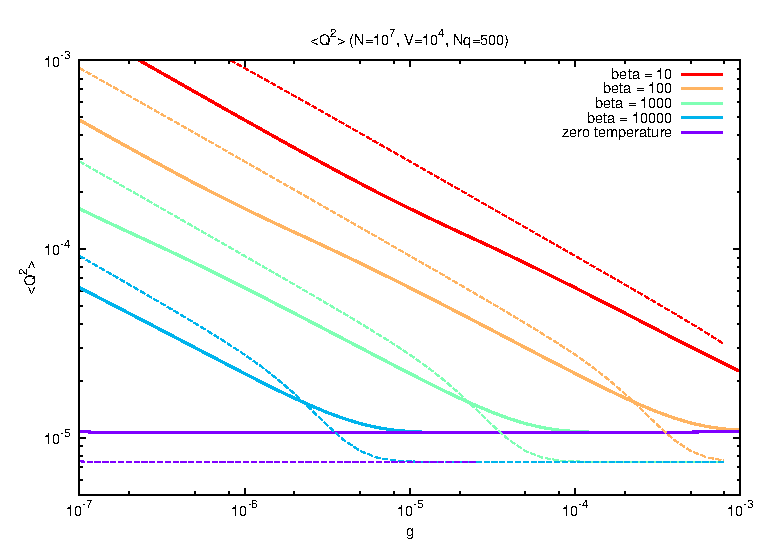
\includegraphics[width = 10cm]{./EPS/Q2.eps}
  \label{Q2}
\end{figure}
\begin{figure}[htbp]
  \centering
  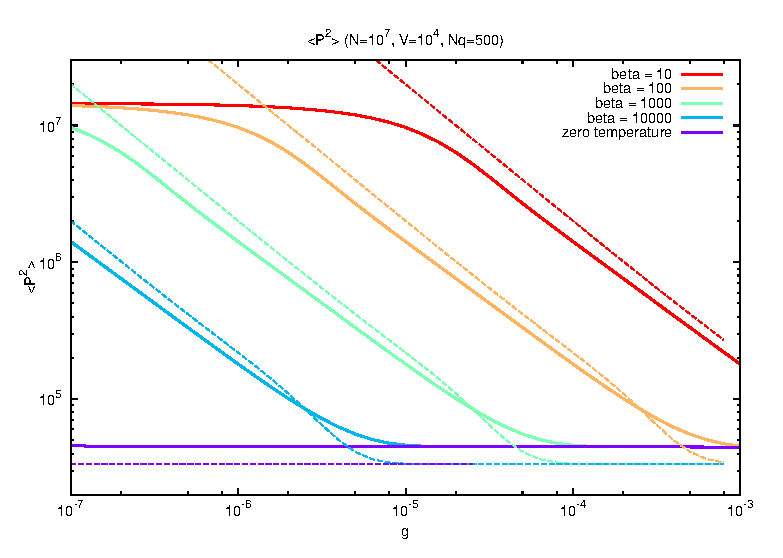
\includegraphics[width = 10cm]{./EPS/P2.eps}
  \label{P2}
\end{figure}
\\\\\\\\\\\\
図\ref{Q2},\ref{P2}\ :\ 破線は各温度に対する変分法による計算結果のプロット.$\ev{Q^2},\ev{P^2}$共に冪についてはよく一致している.

高温領域で位相ゆらぎ$\Delta Q = \sqrt{\ev{Q^2}}$,凝縮粒子数ゆらぎ$\Delta P = \sqrt{\ev{P^2}}$が増加する振る舞いは直感と一致している.

